\chapter{Introducción}

%%%%%%%%%%%%%%%%%%%%%%%%%%%%%%%%%%%%%%%%%%%%%%%%%%%%%%%%%%%%%%%%%%%
\section{Concepto de adherencia terapéutica}
En el ámbito científico, concretamente en el sector sanitario, existen distintos términos utilizados para describir las malas conductas, hábitos o formas no adecuadas de seguir las instrucciones y/o recomendaciones recibidas por parte de los profesionales de la salud. Sin embargo, ``adherencia'' es el término usado como referencia por la Organización Mundial de la Salud (OMS), y se define como el grado en que la conducta de un paciente, en relación con la toma de medicación, el seguimiento de una dieta o la modificación en los hábitos de vida, se ajusta o corresponde con las recomendaciones acordadas con el profesional sanitario. \cite{who2003adherence} 

A menudo se ha utilizado de manera intercambiable \cite{ibarra2017adherencia} junto al término ``cumplimiento", el cual hace alusión a la medida en la que un paciente actúa de acuerdo con la dosis, pauta posológica y plazo prescrito \cite{farmaindustria2023adherencia}. Con todo, la adherencia comprende una aplicación más amplia que incluye todo el espectro del plan terapéutico, tanto en aspectos farmacológicos como no farmacológicos \cite{libroblanco2021}. \\ 

Desde sus inicios, las conceptualizaciones del término adherencia abarcaban una variedad de prácticas recomendadas, que incluían desde el cumplimiento de la medicación hasta ajustes en la dieta y otros cambios de estilo de vida, siempre en línea con las prescripciones indicadas. No obstante, estas conceptualizaciones no siempre reflejaban una verdadera sintonía entre las expectativas del profesional sanitario y la participación del paciente, como lo señaló el médico y epidemiólogo clínico Robert B. Haynes en 1979 \cite{libroblanco2021}. En este sentido, la adherencia no farmacológica cobra especial relevancia al enfatizar la importancia de mantener hábitos saludables, como una dieta adecuada, el cese del consumo de tabaco y otras sustancias nocivas, así como la práctica regular de ejercicio físico. \\

A pesar de las diferencias entre adherencia y cumplimiento, actualmente se acepta cada vez más que la adherencia prevalece sobre el mero cumplimiento de las indicaciones, permitiendo enfrentar de manera más integral el desafío de la adherencia terapéutica \cite{farmaindustria2023adherencia}.


%%%%%%%%%%%%%%%%%%%%%%%%%%%%%%%%%%%%%%%%%%%%%%%%%%%%%%%%%%%%%%%%%%%
\section{Predictores de la adherencia y no adherencia}

El proceso de adherencia se divide en tres etapas: \textbf{iniciación}, cuando el paciente comienza el tratamiento; \textbf{ejecución}, que se refiere al cumplimiento continuo del régimen prescrito; y \textbf{discontinuación}, que ocurre cuando el tratamiento se interrumpe antes de lo indicado. 

Interrupciones como el retraso en empezar el tratamiento o la finalización prematura son ejemplos de fallas en la adherencia que pueden darse en cualquier fase del proceso. No obstante, existe una serie de situaciones que determinan la buena o mala adherencia del paciente, las cuales están ligadas a diferentes factores relacionados con el tratamiento, la sociedad y el sistema sanitario.\\

En lo que respecta al tratamiento, la incertidumbre generada por el desconocimiento acerca de lo recetado conlleva a una peor adherencia, destacando el impacto que generan los efectos adversos, entre otros. Diversos estudios han demostrado la existencia de una relación entre el número y frecuencia de dosis y el cumplimiento farmacológico, de tal forma que este último se consigue garantizar si el número de dosis es bajo, preferiblemente siendo una única dosis diaria. En otros casos se ve afectado y no se obtiene con pautas de más de dos dosis diarias \cite{Claxton2001}. \\

En cuanto a los factores relacionados con la sociedad, unos recursos económicos escasos y el precio elevado de los medicamentos, en el caso de un tratamiento farmacológico, están directamente asociados a una peor adherencia. Por lo contrario, la adherencia mejora cuando el paciente convive con miembros familiares \cite{libroblanco2021}. Está también comprobado que el inicio del proceso de adopción de un hábito de vida impuesto por un profesional sanitario se ve facilitado si el paciente se encuentra rodeado de familiares y amistades que apoyen e inciten su cumplimiento.\\

Uno de los factores más influyentes en la adherencia es la relación entre el profesional sanitario y el paciente, especialmente en el modelo actual de atención centrada en el paciente, donde se promueve la toma de decisiones compartida. En este enfoque el paciente participa activamente en las decisiones relacionadas con su diagnóstico, tratamiento y rehabilitación, permitiéndole expresar sus preferencias, valores y preocupaciones. Sin embargo, su grado de participación en la práctica puede variar según varios factores. Situaciones de emergencia o tratamientos complejos pueden limitar la capacidad del paciente para involucrarse en decisiones críticas. Asimismo, la actitud del profesional sanitario y su disposición para fomentar la participación, así como el nivel de comprensión del paciente y sus preferencias personales, influyen en la medida en que el paciente asume un rol activo. Aun así, la presencia empática y colaborativa del profesional es fundamental durante todo el proceso, mejorando la adherencia y fomentando una relación de confianza. \cite{libroblanco2021}
\newpage

%%%%%%%%%%%%%%%%%%%%%%%%%%%%%%%%%%%%%%%%%%%%%%%%%%%%%%%%%%%%%%%%%%%
\section{Formas de incumplir el tratamiento}

Las categorías más comunes de incumplimiento del tratamiento, que reflejan los distintos comportamientos de los pacientes en relación con la adherencia a sus medicamentos y terapias prescritas, se describen a continuación \cite{ibarra2017adherencia}: 

\begin{itemize}
	\item \textbf{Incumplimiento parcial.} El paciente no sigue el tratamiento de manera constante, únicamente en algunos momentos.

	\item \textbf{Incumplimiento esporádico.} El paciente omite el tratamiento de manera ocasional, lo cual es más frecuente en personas mayores que pueden olvidar dosis o reduirlas debido a preocupaciones sobre posibles efectos adversos
	
	\item \textbf{Incumplimiento secuencial.} El paciente interrumpe el tratamiento durante los periodos en los que se siente bien, reanudándolo sólo cuando los síntomas reaparecen. Este patrón es comparable a lo que se conoce por ``vacaciones terapéuticas".
	
	\item \textbf{Cumplimiento de bata blanca.} El paciente se adhiere al tratamiento únicamente en los días cercanos a las visitas médicas. Este comportamiento, junto con el incumplimiento secuencial, es común en enfermedades crónicas como la hipertensión o la dislipemia.
	
	\item \textbf{Incumplimiento completo.} El paciente abandona el tratamiento de manera indefinida. Este tipo de falta de adherencia es más prevalente entre los jóvenes con enfermedades crónicas, probablemente debido a que los beneficios del tratamiento son a largo plazo, mientras que los costos y efectos adversos son inmediatos.
	
\end{itemize}

%%%%%%%%%%%%%%%%%%%%%%%%%%%%%%%%%%%%%%%%%%%%%%%%%%%%%%%%%%%%%%%%%%%
\section{Métodos de seguimiento y estimación de la adherencia}

Medir la adherencia permite a los profesionales de la salud evaluar hasta qué punto los pacientes siguen las prescripciones de medicamentos según lo indicado. Este proceso de medición puede llevarse a cabo mediante varios métodos, cada uno con sus propias ventajas y limitaciones, desde análisis bioquímicos hasta sistemas electrónicos y cuestionarios. La elección del método adecuado depende de varios factores, incluidos el costo, la facilidad de implementación y la precisión requerida en la medición. \\

Es importante destacar que ningún método es perfecto por sí solo; por ello, combinar varios métodos puede proporcionar una evaluación más completa y precisa de la adherencia. Además, la medición sistemática de la adherencia permite identificar barreras específicas que enfrentan los pacientes. \cite{ibarra2017adherencia}\\
  
\newpage

En las siguientes tablas se muestran los métodos más usados por los farmacéuticos: \\

\begin{table}[ht]
	\centering
	\label{my-label}
	\begin{tabular}{|p{4cm}|p{5.5cm}|p{5.5cm}|}
		\hline
		\textbf{Método} & \textbf{Ventajas} & \textbf{Definición} \\ \hline
		Determinación plasmática & 
		\begin{itemize}
			\item Método directo
			\item Detecta toxicidad
			\item Ventaja en población con farmacocinética alterada (embarazo o disfunción hepática)
		\end{itemize} & 
		\begin{itemize}
			\item Caro e invasivo
			\item Recogida e interpretación no estandarizadas
		\end{itemize} \\ \hline
		Registros de dispensación & 
		\begin{itemize}
			\item Fácil obtención de datos
			\item Correlación moderada con resultados
		\end{itemize} & 
		\begin{itemize}
			\item Sobrestimación
			\item No mide la frecuencia horaria
			\item Asume que la recogida de medicación equivale a adherencia
			\item No distingue tipos de adherencia
		\end{itemize} \\ \hline
		Recuento de medicación & 
		\begin{itemize}
			\item Bajo costo
			\item Correlación moderada con resultados
		\end{itemize} & 
		\begin{itemize}
			\item Requiere colaboración del paciente
			\item Sobrestimación
			\item Asume que el paciente no almacena medicación
		\end{itemize} \\ \hline
	\end{tabular}

\caption{Métodos de estimación de la adherencia (I).}
\end{table}

Por ejemplo, los análisis bioquímicos pueden confirmar la presencia de un fármaco en el organismo, pero no indican si se sigue la pauta de dosis exacta. En cambio, los sistemas electrónicos y los cuestionarios permiten monitorear patrones de consumo a lo largo del tiempo, aunque pueden estar sujetos a sesgos de autoinforme o problemas técnicos. La medición de la adherencia es, por tanto, un desafío complejo que requiere un enfoque equilibrado para obtener información útil y confiable \cite{ibarra2017adherencia}.

\newpage

\begin{table}[ht]
	\centering
	\label{my-label}
	\begin{tabular}{|p{4cm}|p{5.5cm}|p{5.5cm}|}
		\hline
		\textbf{Método} & \textbf{Ventajas} & \textbf{Definición} \\ \hline
MEMS/dispositivos electrónicos & 
\begin{itemize}
	\item Patrones de adherencia en el tiempo
	\item Análisis detallado
\end{itemize} & 
\begin{itemize}
	\item Costoso
	\item Infraestimación
	\item No disponible en todos los centros
	\item Vulnerable a fallos tecnológicos
\end{itemize} \\ \hline
Cuestionario/adherencia autorreferida & 
\begin{itemize}
	\item Bajo costo
	\item Fácil de implementar
\end{itemize} & 
\begin{itemize}
	\item No estandarizado
	\item Sobrestimación
	\item Sensibilidad baja
\end{itemize} \\ \hline
	\end{tabular}

\caption{Métodos de estimación de la adherencia (II).}
\end{table}

La figura inferior es un cuestionario ARMS-e diseñado para medir la adherencia en pacientes con múltiples patologías. Este instrumento evalúa la falta de adherencia de forma multidimensional, lo que permite personalizar las intervenciones según las barreras detectadas en cada individuo. Consta de 12 preguntas y no define un punto de corte específico; en su lugar, una puntuación más baja refleja una mejor adherencia. Para cuantificar el grado de adherencia, a cada opción de respuesta se le asigna un valor de 1 a 4, siguiendo una escala Likert: nunca, algunas veces, casi siempre o siempre. \cite{pages2018metodos}

\begin{figure}[h!]
	\centering
	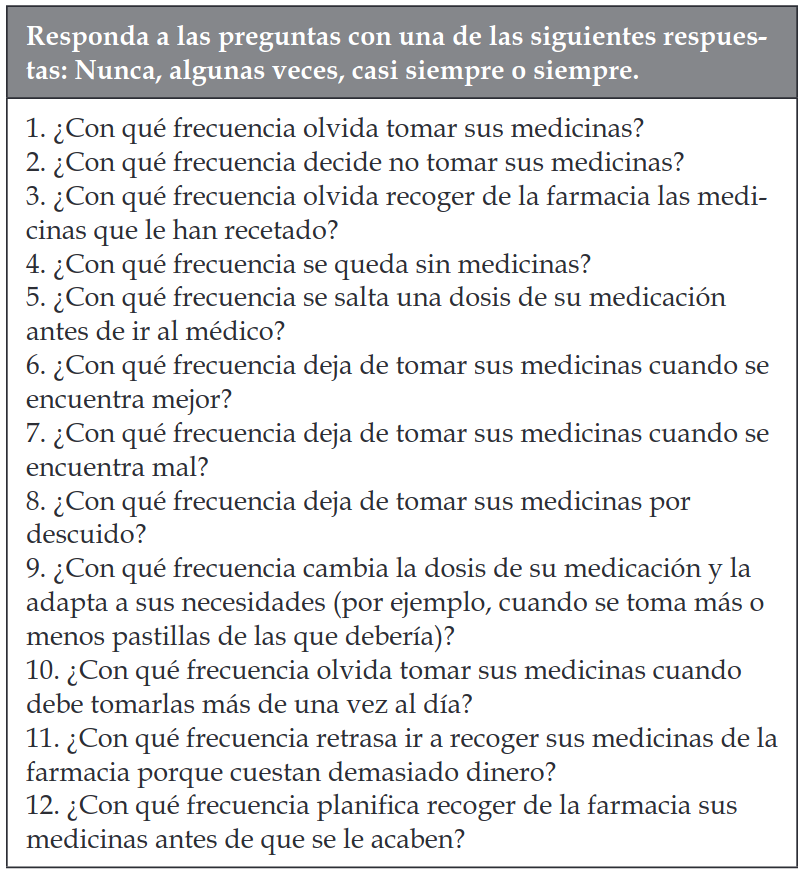
\includegraphics[width=0.52\textwidth]{imagenes/cuestionario_adherencia.png}
	\caption{Cuestionario de adherencia.}
	\label{fig:cuestionario_adherencia}
\end{figure}


%%%%%%%%%%%%%%%%%%%%%%%%%%%%%%%%%%%%%%%%%%%%%%%%%%%%%%%%%%%%%%%%%%%
\section{Estado del arte: iniciativas y programas desarrollados}
A nivel nacional se encuentran en fase de implantación varios proyectos que posibilitan el servicio de seguimiento farmacoterapéutico \cite{CONTHE2014336}, como es el caso del programa conSIGUE \cite{programa_consigue}, cuyo objetivo es evaluar y mejorar la adherencia terapéutica en personas mayores, con enfermedades crónicas, polimedicadas e incumplidoras. También existe el programa Adhiérete \cite{programa_adhierete_2015}, similar al anterior, y que aprovecha los sistemas personalizados de dosificación para ofrecer un servicio de asistencia domiciliaria y de evaluación personalizada de la calidad de vida del paciente. \\
A pesar de mostrar resultados favorecedores, se trata de sistemas diseñados y puestos en funcionamiento hace más de una década, orientados mayoritariamente a personas de la tercera edad y pacientes polimedicados y crónicos, sin disponer de plataformas digitales para poder estar al alcance de más rangos de edad. \\

Un ejemplo de programa que combina las técnicas clásicas con el soporte digital es HazAdherencia, el cual facilita a los colegiados la formación y los medios necesarios para poder atender y prestar asistencia farmacéutica personalizada a pacientes con hipertensión arterial, diabetes o dislipemia \cite{hazadherencia2024}. Aunque se tengan las herramientas digitales necesarias, su uso no está dirigido hacia todo tipo de pacientes. \\

Existen también aplicaciones no oficiales que organizan y alertan sobre la toma de medicación, abiertas a todo el público, pero sin soporte por parte de los profesionales de la salud.  \\



%%%%%%%%%%%%%%%%%%%%%%%%%%%%%%%%%%%%%%%%%%%%%%%%%%%%%%%%%%%%%%%%%%%
\section{Motivación}

La correcta adherencia a los tratamientos médicos es esencial para garantizar su eficacia. Un cumplimiento deficiente puede llevar a resultados adversos en la salud, incrementar los costos asociados al manejo de la enfermedad y afectar negativamente el ámbito social, tanto a nivel individual como colectivo.

\begin{itemize}
	\item \textbf{Impactos en la salud.} Los medicamentos que han probado su eficacia en ensayos clínicos podrían no ser efectivos en la práctica clínica si no se administran correctamente. Esto incluye tanto las recomendaciones farmacológicas como las no farmacológicas. La reducción en la eficacia depende del nivel de incumplimiento, las características específicas de la enfermedad, las propiedades farmacodinámicas y farmacocinéticas del fármaco, y la condición preexistente del paciente. \cite{libroblanco2021} 
	
	\item \textbf{Implicaciones económicas.} La falta de adherencia se asocia con un incremento en la severidad de las enfermedades, un mayor número de visitas médicas no planificadas, el uso de medicamentos no necesarios y hospitalizaciones, lo cual eleva los gastos de salud significativamente en casos de enfermedades crónicas. Además, los costes indirectos comprenden la pérdida de productividad laboral de los enfermos y sus cuidadores. \cite{libroblanco2021}
\end{itemize}

Dado que el problema de la falta de adherencia está generalizado y se contempla en más rangos de edad, este proyecto propone un seguimiento y mejora de la adherencia terapéutica para todo tipo de pacientes mediante la creación de un medio digital actual y moderno que facilite a los farmacéuticos la elaboración, preparación y seguimiento de cualquier tipo de tratamiento, así como la recomendación y advertencia sobre la toma de la medicación, si está incluida, de acuerdo a directrices específicas.

%%%%%%%%%%%%%%%%%%%%%%%%%%%%%%%%%%%%%%%%%%%%%%%%%%%%%%%%%%%%%%%%%%%
\section{Objetivos}
Los objetivos principales de este proyecto se enumeran como sigue:
\begin{enumerate}
	\item Ofrecer una atención personalizada a cada paciente, recogiendo información acerca de su estado de salud y recomendaciones sanitarias.
	
	\item Proporcionar información sobre medicación y obtener retroalimentación por parte de los pacientes para posibilitar a los farmacéuticos la labor de realizar un seguimiento del tratamiento vigente.
	
	\item Recordar los tratamientos y hábitos impuestos.
	
	\item Medir la adherencia del paciente mediante una adaptación de los métodos tradicionales.
	
	\item Ofrecer estadísticas acerca de la adherencia terapéutica.
	
	\item Favorecer la relación profesional-paciente mediante un contacto continuo entre ambos.
\end{enumerate}
	


%%%%%%%%%%%%%%%%%%%%%%%%%%%%%%%%%%%%%%%%%%%%%%%%%%%%%%%%%%%%%%%%%%%